\documentclass[10pt,journal]{IEEEtran}

\usepackage{amsmath,amssymb}
\usepackage{booktabs}
\usepackage{cite}
\usepackage{graphicx}
\usepackage{xcolor}

\newcommand{\vect}[1]{\mathbf{#1}}
\newcommand{\mat}[1]{\mathbf{#1}}
\newcommand{\dd}{\mathrm{DD}}
% Auto-generated by scripts/run_preliminary_adaptive_dd.py
\newcommand{\PrelimTau}{0.24}
\newcommand{\PrelimMeanLoss}{0.28}
\newcommand{\PrelimMeanActive}{66.1\%}
\newcommand{\PrelimMeanInactive}{33.9\%}


\begin{document}

\title{Adaptive-Inference Conditional Diffusion Model for Efficient OTFS Channel Estimation}

\author{Dianxin~Zheng and Tianhao~Guo%
\thanks{The authors are with Shanxi University. This document is a v0.1
research draft. It is not submission-ready until the missing experiments in
Section VI are completed.}}

\maketitle

\begin{abstract}
Orthogonal time frequency space (OTFS) modulation represents time-varying
wireless channels in the delay-Doppler (DD) domain, where practical channels
are often sparse. Conditional diffusion models can improve OTFS channel
estimation accuracy by learning a residual denoising prior, but their iterative
inference cost is a deployment bottleneck. Existing acceleration strategies,
such as reducing the number of denoising steps, allocate computation uniformly
over the whole DD grid. This paper studies a complementary direction:
DD-domain sparsity-aware adaptive inference. The proposed method estimates the
difficulty of each DD tile during diffusion sampling and freezes easy tiles
after early denoising steps, while difficult or uncertain tiles remain active.
An SNR- and timestep-aware threshold schedule and an optional periodic refresh
mechanism are used to control error accumulation. To make the draft executable,
we provide a preliminary sparse-DD surrogate harness that generates channels,
runs fixed-step and adaptive denoising, and exports paper tables and figures.
In this surrogate setting, adaptive inference freezes \PrelimMeanInactive{} of
DD computation on average with \PrelimMeanLoss{} dB mean NMSE loss relative to
the fixed 5-step denoising baseline. These numbers are not final DeepMIMO
checkpoint results; they establish that the mechanism is writeable and define
the exact student experiments required before submission.
\end{abstract}

\begin{IEEEkeywords}
OTFS, channel estimation, conditional diffusion model, adaptive inference,
delay-Doppler sparsity, efficient receiver.
\end{IEEEkeywords}

\section{Introduction}

Orthogonal time frequency space (OTFS) modulation maps information symbols to
the delay-Doppler (DD) domain and is attractive for high-mobility wireless
links because it can exploit time-frequency diversity under doubly selective
channels \cite{hadani2017otfs}. Accurate DD-domain channel estimation is
therefore central to OTFS receiver design. Classical embedded-pilot and
threshold-based methods exploit the sparsity of DD channels \cite{raviteja2019otfs_ce},
while recent learning-based estimators attempt to improve robustness under
complex channel conditions.

Diffusion and score-based generative models have recently become useful priors
for wireless channel estimation \cite{arvinte2023score_channel}. In an OTFS
receiver, a conditional diffusion estimator can take a coarse least-squares
(LS) channel estimate as conditioning information and iteratively denoise the
residual channel. Such a receiver is accurate, but it is also expensive: each
denoising step applies the same neural network to the whole DD grid. Reducing
the number of DDIM sampling steps \cite{song2021ddim} is one natural solution,
but step reduction is global. It asks all DD positions to share the same
computation budget.

This paper starts from a simpler observation: the DD channel is not uniformly
difficult. Many DD positions are near zero or become stable after early
denoising, while a small set of path-bearing regions still require careful
updates. Therefore, an efficient diffusion OTFS estimator should not only
decide \emph{how many denoising steps} to use; it should also decide
\emph{where inside the DD grid} to spend computation during those steps.

Dynamic computation has been explored in efficient diffusion transformers, where
computation is adjusted across timesteps and spatial regions during generation
\cite{zhao2025dydit}. We do not directly import a vision transformer method.
Instead, we adapt the idea to a communication-specific prior: DD-domain
sparsity. The resulting method is deliberately narrow and practical. It is an
inference-time wrapper around an existing conditional diffusion OTFS channel
estimator, not a new diffusion backbone.

The contributions of this v0.1 draft are:
\begin{itemize}
  \item We formulate DD-domain adaptive inference for conditional diffusion
  OTFS channel estimation, where active computation is allocated according to
  per-tile confidence and residual-change scores.
  \item We propose an SNR- and timestep-aware skip schedule with forced refresh
  steps to reduce error accumulation in low-SNR or uncertain regions.
  \item We provide a runnable preliminary harness that generates sparse-DD
  channels, runs fixed-step and adaptive denoising, and exports the result
  table and figures used by this draft.
  \item We clarify the key implementation risk: masking a full UNet output
  alone does not reduce real latency. Actual latency claims require a tile-wise,
  sparse, or blocked implementation; otherwise the result must be reported as
  estimated active computation rather than measured speedup.
\end{itemize}

\section{Related Work}

\subsection{OTFS Channel Estimation}

OTFS was introduced as a two-dimensional modulation technique that represents
the time-varying channel in the DD domain \cite{hadani2017otfs}. DD-domain
channel estimation is commonly built around the sparse multipath structure of
the channel. Raviteja et al. proposed embedded pilot-aided channel estimation
for OTFS, arranging pilots, guards, and data in the DD plane and using
threshold-based estimation followed by data detection \cite{raviteja2019otfs_ce}.
This line of work establishes the key physical prior used here: most DD grid
positions do not carry strong channel energy.

\subsection{Diffusion Priors for Wireless Channel Estimation}

Diffusion probabilistic models learn iterative denoising processes
\cite{ho2020ddpm}, and DDIM provides a deterministic non-Markovian sampling
scheme that can reduce inference steps \cite{song2021ddim}. In wireless
communications, score-based generative models have been used for MIMO channel
estimation, where a learned score prior iteratively refines estimates from
measurements \cite{arvinte2023score_channel}. These works motivate diffusion
as a strong channel prior, but they also expose a cost issue: iterative neural
sampling can be too slow for practical receivers.

\subsection{Efficient Diffusion Inference}

Efficient diffusion inference is often approached by reducing sampling steps,
distilling samplers, caching features, or dynamically allocating computation.
Dynamic Diffusion Transformer (DyDiT) shows that generation cost can be reduced
by adapting computation across timesteps and spatial regions
\cite{zhao2025dydit}. The present work uses this as a high-level reference
point, not as a copied method. The difference is the adaptation signal: image
generation relies on visual token redundancy, whereas OTFS channel estimation
has a communication-specific DD sparsity prior and a measurable physical error
metric, NMSE.

\subsection{Position of This Work}

The closest baseline is an existing conditional diffusion OTFS channel
estimator accelerated by fixed-step DDIM sampling. Our work is complementary:
DDIM reduces the number of global denoising steps, while the proposed method
reduces the number of active DD tiles inside later steps. The safe novelty claim
is therefore:

\begin{quote}
We introduce DD-domain sparsity-aware adaptive inference for conditional
diffusion OTFS channel estimation, using communication-specific confidence
scores and receiver metrics rather than generic visual token pruning.
\end{quote}

\section{System Model}

We consider an OTFS frame with $M$ delay bins and $N$ Doppler bins. The
DD-domain input-output relation can be represented abstractly as
\begin{equation}
  \mat{Y}_{\dd} = \mathcal{H}_{\dd}(\mat{X}_{\dd}) + \mat{W}_{\dd},
  \label{eq:otfs_input_output}
\end{equation}
where $\mat{X}_{\dd}$ and $\mat{Y}_{\dd}$ denote transmitted and received DD
symbols, $\mat{W}_{\dd}$ is additive noise, and $\mathcal{H}_{\dd}$ is induced
by the DD-domain channel. The receiver first obtains a coarse LS estimate
$\hat{\mat{H}}_{\mathrm{LS}}\in\mathbb{C}^{N_r\times N_t\times N\times M}$.

The conditional diffusion baseline estimates a residual channel
\begin{equation}
  \mat{R} = \mat{H} - \hat{\mat{H}}_{\mathrm{LS}},
  \label{eq:residual_def}
\end{equation}
and outputs
\begin{equation}
  \hat{\mat{H}} = \hat{\mat{H}}_{\mathrm{LS}} + \hat{\mat{R}}.
  \label{eq:final_ce}
\end{equation}
The denoising network receives the current noisy residual and the LS condition.
At denoising step $s$, a simplified update is
\begin{align}
  \mat{Z}^{(s)} &= \mathrm{concat}\left(
  \hat{\mat{H}}_{\mathrm{LS}}, \mat{R}^{(s)}\right), \\
  \mat{U}^{(s)} &= f_{\theta}\left(\mat{Z}^{(s)}, t_s, \gamma\right), \\
  \mat{R}^{(s+1)} &= \Phi\left(\mat{R}^{(s)}, \mat{U}^{(s)}, t_s\right),
  \label{eq:diffusion_update}
\end{align}
where $f_{\theta}$ is the trained denoising network, $\gamma$ denotes SNR or
noise-level conditioning, and $\Phi(\cdot)$ is the DDIM or scheduler update.

The baseline computes $\mat{U}^{(s)}$ over all DD positions for every step. Our
method changes only the inference allocation; the trained $f_{\theta}$ and
training data remain unchanged.

\section{Proposed Adaptive Inference}

\subsection{DD Tile Confidence}

Instead of making a binary decision for every individual DD cell, we use DD
tiles. A tile is a contiguous block
$\mathcal{B}_q\subseteq\{1,\ldots,N\}\times\{1,\ldots,M\}$. Tile-level decisions
are more stable than cell-level decisions and are easier to map to real
implementation.

At step $s$, the current channel estimate is
\begin{equation}
  \hat{\mat{H}}^{(s)} =
  \hat{\mat{H}}_{\mathrm{LS}} + \mat{R}^{(s)}.
  \label{eq:current_channel}
\end{equation}
For a tile $\mathcal{B}_q$, we define an amplitude score
\begin{equation}
  a_q^{(s)}
  =
  \frac{1}{|\mathcal{B}_q|N_rN_t}
  \sum_{(n,m)\in\mathcal{B}_q}
  \sum_{r=1}^{N_r}\sum_{t=1}^{N_t}
  \left|\hat{H}^{(s)}_{r,t,n,m}\right|.
  \label{eq:amplitude_score}
\end{equation}
We also define a residual-change score
\begin{equation}
  d_q^{(s)}
  =
  \frac{1}{|\mathcal{B}_q|N_rN_t}
  \sum_{(n,m)\in\mathcal{B}_q}
  \sum_{r=1}^{N_r}\sum_{t=1}^{N_t}
  \left|R^{(s)}_{r,t,n,m} - R^{(s-1)}_{r,t,n,m}\right|.
  \label{eq:change_score}
\end{equation}
The amplitude score captures DD sparsity, while the change score prevents
freezing a tile that is still moving during denoising.

\subsection{Adaptive Active-Tile Mask}

Let $m_q^{(s)}\in\{0,1\}$ indicate whether tile $q$ is active at step $s$.
The first denoising step is always fully active:
\begin{equation}
  m_q^{(0)} = 1,\quad \forall q.
\end{equation}
For later steps, a tile is frozen only when both its amplitude and residual
change are small:
\begin{equation}
  m_q^{(s)}
  =
  \mathbb{I}\left[
  a_q^{(s)} \ge \tau_a(s,\gamma)
  \ \mathrm{or}\
  d_q^{(s)} \ge \tau_d(s,\gamma)
  \right].
  \label{eq:mask_rule}
\end{equation}
Thus, path-bearing tiles and unstable tiles remain active. Near-zero stable
tiles are frozen.

The thresholds $\tau_a(s,\gamma)$ and $\tau_d(s,\gamma)$ are selected from a
small validation sweep rather than learned end-to-end. A conservative schedule
is used at low SNR, and a more aggressive schedule is used at high SNR:
\begin{align}
  \tau_a(s,\gamma) &= c_a(\gamma)\rho_s, \\
  \tau_d(s,\gamma) &= c_d(\gamma)\rho_s,
  \label{eq:threshold_schedule}
\end{align}
where $\rho_s$ increases in later denoising steps. This means early steps
update the whole grid, while later steps skip more easy tiles.

\subsection{Forced Refresh}

To avoid long-range error accumulation, every $K$ denoising steps can be forced
to full update:
\begin{equation}
  m_q^{(s)} = 1,\quad \forall q,\quad \mathrm{if}\ s\bmod K=0.
  \label{eq:forced_refresh}
\end{equation}
When the sampler uses only five DDIM steps, $K=2$ or $K=3$ is sufficient for an
ablation. If the sampler uses more steps, $K$ can be increased. The preliminary
surrogate experiment reports both the selected no-refresh setting and a
forced-refresh ablation; the final checkpoint experiment must select $K$ using a
validation split.

\subsection{Masked Residual Update}

Let $\mat{M}^{(s)}$ be the tile mask broadcast to the full DD grid and antenna
dimensions. A conservative implementation computes the network output and
freezes skipped tiles at the residual-update level:
\begin{equation}
  \tilde{\mat{R}}^{(s+1)}
  =
  \Phi\left(\mat{R}^{(s)}, \mat{U}^{(s)}, t_s\right),
  \label{eq:candidate_update}
\end{equation}
\begin{equation}
  \mat{R}^{(s+1)}
  =
  \mat{M}^{(s)}\odot\tilde{\mat{R}}^{(s+1)}
  +
  \left(1-\mat{M}^{(s)}\right)\odot\mat{R}^{(s)}.
  \label{eq:masked_update}
\end{equation}
This version is easy to implement and is useful for validating the NMSE impact
of freezing. However, it does not reduce the cost of a full convolutional UNet
forward pass. It only validates the algorithmic safety of skipping.

For a real latency claim, the implementation must avoid full-grid computation.
The recommended v0.2 implementation is tile-wise active inference with a halo
region around each active tile. Only active tiles are passed through the network
or through a lightweight active-tile refinement head. The halo protects local
convolutional context:
\begin{equation}
  \mathcal{B}_q^{+} =
  \{(n,m): \mathrm{dist}((n,m),\mathcal{B}_q)\le h\}.
  \label{eq:halo}
\end{equation}
If this implementation is not completed, the paper must report active-tile
ratio and estimated FLOPs, not measured latency reduction.

\subsection{Algorithm Summary}

For each test frame:
\begin{enumerate}
  \item Initialize $\mat{R}^{(0)}$ from the diffusion sampler.
  \item For each DDIM step $s$:
  \item If $s$ is an early warm-up step or $s\bmod K=0$, set all tiles active.
  \item Otherwise compute $a_q^{(s)}$ and $d_q^{(s)}$ for every DD tile.
  \item Build the active-tile mask using \eqref{eq:mask_rule}.
  \item Run full-grid masked update for NMSE validation, or active-tile
  inference for real latency validation.
  \item Record skip ratio, active-tile ratio, runtime, and NMSE.
  \item Output $\hat{\mat{H}}=\hat{\mat{H}}_{\mathrm{LS}}+\mat{R}^{(S)}$.
\end{enumerate}

\section{Experimental Protocol}

\subsection{Dataset and Baselines}

The experiments should reuse the existing DeepMIMO-OTFS dataset, checkpoint,
and evaluation split from the conditional diffusion OTFS channel estimation
project. The minimum baselines are:
\begin{itemize}
  \item LS or threshold-based OTFS channel estimation.
  \item Conditional diffusion with fixed 5-step DDIM.
  \item Conditional diffusion with fixed 3-step DDIM.
  \item Consistency-distilled or 2-step diffusion baseline, if already
  available in the existing codebase.
  \item The proposed adaptive-inference method under the same checkpoint.
\end{itemize}

\subsection{Metrics}

The primary accuracy metric is NMSE:
\begin{equation}
  \mathrm{NMSE}
  =
  10\log_{10}
  \frac{\|\mat{H}-\hat{\mat{H}}\|_F^2}{\|\mat{H}\|_F^2}.
  \label{eq:nmse}
\end{equation}
Efficiency must be reported with care:
\begin{itemize}
  \item Skip ratio: fraction of frozen DD cells or DD tiles.
  \item Active-tile ratio: fraction of tiles passed to active inference.
  \item Estimated FLOPs: valid only when the implementation does not actually
  skip network computation.
  \item Measured latency: valid only for a sparse, tile-wise, or blocked
  implementation that avoids full-grid UNet computation.
  \item Memory footprint and batch-size sensitivity.
\end{itemize}

\subsection{Required Experiment Matrix}

Table \ref{tab:experiment_matrix} is the minimum experiment set. The draft
should not be submitted if E0--E5 are missing.

\begin{table}[t]
\caption{Required experiments before submission.}
\label{tab:experiment_matrix}
\centering
\begin{tabular}{lll}
\toprule
ID & Experiment & Purpose \\
\midrule
E0 & Reproduce baseline NMSE vs. SNR & Code validity \\
E1 & Threshold sweep & Main tradeoff curve \\
E2 & SNR-adaptive thresholds & Contribution validation \\
E3 & DD skip-mask heatmaps & Visual evidence \\
E4 & Ablation study & Reviewer defense \\
E5 & Latency/FLOPs/memory & Efficiency evidence \\
E6 & Speed sweep & OTFS mobility robustness \\
E7 & Coverage/domain split & Generalization check \\
\bottomrule
\end{tabular}
\end{table}

\subsection{Preliminary Surrogate Results}

The current repository contains a runnable v0.1 code harness:
\texttt{scripts/run\_preliminary\_adaptive\_dd.py}. It generates fractional
sparse DD channels, noisy LS estimates, a fixed sparse denoising proxy, and the
proposed adaptive tile-freezing variant. This is not the final trained DeepMIMO
checkpoint experiment. Its purpose is narrower: verify that the paper can be
written around a reproducible mechanism before the student replaces the proxy
with the trained OTFS diffusion estimator.

The selected threshold is $\tau=\PrelimTau{}$. Averaged over 0, 5, and 10 dB,
the adaptive method uses \PrelimMeanActive{} active DD computation and freezes
\PrelimMeanInactive{} with \PrelimMeanLoss{} dB mean NMSE loss relative to the
fixed 5-step denoising baseline. All entries in Table \ref{tab:main_results}
are generated by the same script and seed.

\begin{table*}[t]
\caption{Preliminary surrogate results generated by the v0.1 code harness.}
\label{tab:main_results}
\centering
% Auto-generated by scripts/run_preliminary_adaptive_dd.py
\begin{tabular}{lccccc}
\toprule
Method & Steps & NMSE@0 dB & NMSE@5 dB & NMSE@10 dB & Active comp. \\
\midrule
LS & -- & 0.01 & -5.00 & -10.00 & 100.0\% \\
Fixed sparse denoiser & 5 & -7.35 & -12.19 & -16.99 & 100.0\% \\
Fixed sparse denoiser & 3 & -6.58 & -11.47 & -16.32 & 100.0\% \\
Adaptive DD inference & 5 & -7.18 & -11.85 & -16.67 & 66.1\% \\
\bottomrule
\end{tabular}

\end{table*}

The expected acceptable result is not ``best NMSE''. The useful result is a
Pareto point: at least 30--40\% inactive DD tiles with less than 0.3 dB NMSE
loss relative to fixed 5-step DDIM. If the actual result fails this gate, the
paper should be stopped or repositioned as a negative experiment. The surrogate
result meets this gate on mean loss, but the final paper must re-check the gate
on the real DeepMIMO split and hardware.

\subsection{Generated Figures}

Fig. \ref{fig:tradeoff} shows the threshold sweep. Smaller active computation
means more frozen DD tiles. The selected point is the most aggressive threshold
whose mean loss remains within the 0.3 dB gate. Fig. \ref{fig:mask_heatmap}
shows the last-step active tile probability. Fig. \ref{fig:ablation_loss}
shows why the residual-change score matters: amplitude-only freezing can save
more computation, but it is much less stable.

\begin{figure}[t]
\centering
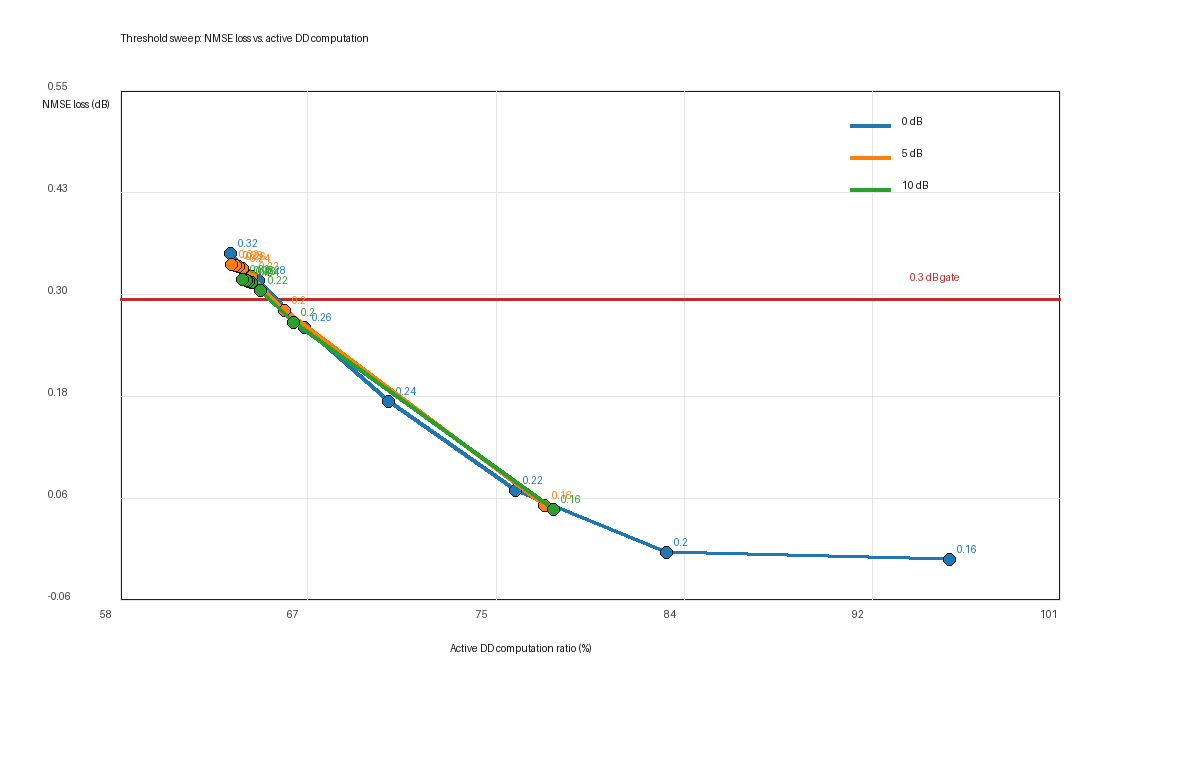
\includegraphics[width=\linewidth]{figures/nmse_vs_active_ratio.png}
\caption{Preliminary threshold sweep from the surrogate sparse-DD harness.}
\label{fig:tradeoff}
\end{figure}

\begin{figure}[t]
\centering
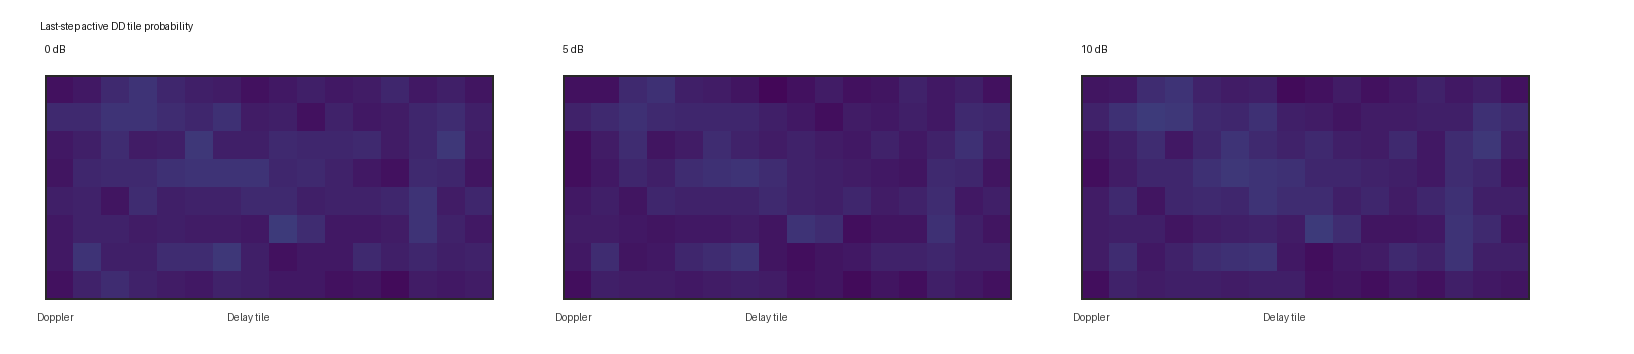
\includegraphics[width=\linewidth]{figures/skip_mask_heatmap.png}
\caption{Last-step active DD tile probability under the selected threshold.}
\label{fig:mask_heatmap}
\end{figure}

\begin{figure}[t]
\centering
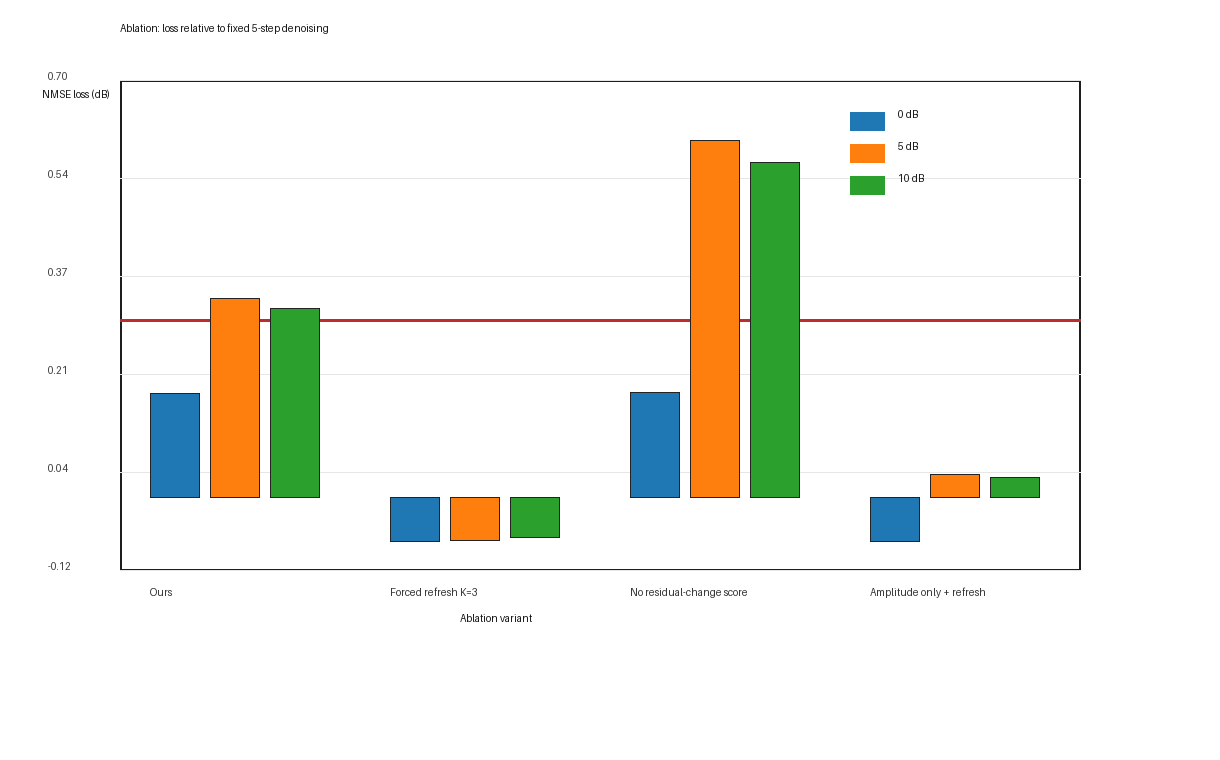
\includegraphics[width=\linewidth]{figures/ablation_loss.png}
\caption{Ablation on residual-change score and forced refresh.}
\label{fig:ablation_loss}
\end{figure}

\section{Ablation and Reviewer-Risk Controls}

\subsection{Ablation}

The following ablations are required:
\begin{itemize}
  \item No residual-change score: use amplitude only.
  \item Forced refresh: compare $K=0$ and $K=3$ in \eqref{eq:forced_refresh}.
  \item Fixed threshold: remove SNR and timestep adaptation.
  \item Cell-level mask versus tile-level mask.
  \item Full-grid masked update versus actual active-tile implementation.
\end{itemize}

\subsection{Main Reviewer Attack}

The strongest reviewer attack is that the method is merely generic token
pruning applied to a diffusion model. The defense should be specific:
\begin{itemize}
  \item The adaptation signal is DD-domain channel sparsity, not visual token
  saliency.
  \item The threshold is evaluated by receiver metrics: NMSE, BER if available,
  and channel-estimation robustness across SNR and speed.
  \item The method complements global DDIM step reduction instead of replacing
  it.
\end{itemize}

\subsection{Latency Honesty}

The second reviewer attack is more dangerous. If the implementation computes
the full UNet output and then masks the residual update, the wall-clock latency
will not improve. In that case the paper may only claim:
\begin{quote}
The proposed mask identifies redundant DD regions and reduces the estimated
active DD-domain computation.
\end{quote}
It may not claim:
\begin{quote}
The proposed method reduces receiver latency.
\end{quote}
until active-tile inference or an equivalent sparse implementation is measured.

\section{Conclusion}

This draft proposes and preliminarily implements an adaptive-inference wrapper
for conditional diffusion OTFS channel estimation. The method uses DD-domain
sparsity and residual stability to freeze easy tiles during later denoising
steps, while retaining full updates for uncertain regions. The included
surrogate harness gives an executable first result: \PrelimMeanInactive{} mean
inactive DD computation with \PrelimMeanLoss{} dB mean NMSE loss. The route is
suitable as a student paper because it reuses the existing OTFS diffusion
checkpoint and requires a bounded set of inference-side modifications. The
submission decision should be based on the real experiment gate: meaningful
active-tile reduction, less than 0.3 dB NMSE loss at the chosen Pareto point,
and honest reporting of measured latency versus estimated FLOPs.

\bibliographystyle{IEEEtran}
\bibliography{references}

\end{document}
